\chapter[Matching matched filtering]{Matching matched filtering using deep networks for gravitational wave astronomy}\label{ch:chap_4}

We note to the reader that this text is a modified version of the 
published paper here~\cite{PhysRevLett.120.141103}. Modifications include: 
the addition of several diagnostic plots and some textual expansion on the 
background of techniques used.

In brief: we report in this chapter on the construction of a deep 
convolutional neural network that can reproduce the 
sensitivity of a matched-filtering search for binary black hole gravitational-wave signals. 
The standard method for the detection of well-modeled transient gravitational-wave signals 
is matched filtering. We use only whitened time series of measured gravitational-wave strain as 
an input, and we train and test on simulated binary black hole signals in synthetic 
Gaussian noise representative of Advanced LIGO sensitivity. We show that our network can 
classify signal from noise with a performance that emulates that of match filtering applied 
to the same datasets when considering the sensitivity defined by receiver-operator characteristics.

%
% Summarise main differences
%


\section{Introduction}
%
% intro to gravitational-waves
%
The field of \ac{GW} astronomy has seen an explosion of \ac{CBC} 
detections over the past several years. The first of these were 
\ac{BBH} detections~\cite{PhysRevLett.116.061102, PhysRevLett.116.241103, PhysRevLett.118.221101,1811.12907,2010.14527}, then the 
first detection of a binary neutron star 
system~\cite{PhysRevLett.119.161101}, as well as
the first \ac{NSBH} detections~\cite{Abbott_2021}. 
This \ac{BNS} event was seen in conjunction with a gamma-ray
burst~\cite{2017arXiv171005834L,2017arXiv171005446G,2017arXiv171005449S} 
and multiple post-merger electromagnetic signatures~\cite{2017arXiv171005833L}. 
These detections were made possible by the 
detectors the \ac{LVK}. Over the coming years many more such 
observations, including \acp{BBH}, \acp{BNS}, \acp{NSBH}, as well as other 
more exotic sources are likely to be observed on a more frequent basis. 
As such, the need for more efficient search methods will be 
more pertinent as the detectors increase in sensitivity.

%
% describe the existing algorithms and their potential limitations
%
The algorithms used by the search pipelines to make
detections of \ac{CBC} signals~\cite{0264-9381-33-21-215004, 0004-637X-748-2-136,PhysRevD.90.082004} are, in general, computationally expensive. The methods used are complex, sophisticated processes computed over a large parameter space using advanced signal processing techniques. The computational cost to run the search analysis is due to the large parameter space, as well as analysis of the high frequency components  of the waveform where high data sample rates are required. Distinguishing noise from signal in these search pipelines is achieved, in part, using a technique known as template based matched-filtering (Sec. ~\ref{sec:matched_filtering}). 

%
% introduce matched-filtering
%
Matched-filtering uses a bank~\cite{PhysRevD.86.084017,
1705.01845,PhysRevD.80.104014, PhysRevD.90.082004, PhysRevD.89.084041} of template waveforms~\cite{PhysRevD.44.3819, PhysRevD.89.061502,
PhysRevD.89.024003, Blanchet2014} each with different component mass
and/or spin values. A template bank will span a large astrophysical parameter space since we do not know a priori the true \ac{GW}s parameter values. Waveform models that cover the inspiral, merger, and ringdown phases of a compact binary coalescence are based on combining post-Newtonian theory~\cite{PhysRevD.84.049901,PhysRevD.80.084043,Blanchet2014,PhysRevD.93.084054}, the effective-one-body formalism~\cite{PhysRevD.59.084006}, and numerical relativity simulations~\cite{PhysRevLett.95.121101}.

%
% introduce deep learning
%
Deep learning is a subset of machine learning which has gained in popularity in recent years~\cite{NIPS2012_4824, 1406.2661, 1409.1556, 1412.7062, 1311.2901, 1409.4842} with the rapid development of \ac{GPU} technology. Some successful implementations of deep learning include image processing~\cite{1603.08511,1412.2306,NIPS2012_4824}, medical
diagnosis~\cite{KONONENKO200189}, and microarray gene expression
classification~\cite{Pirooznia2008}. There has also been
some recent success in the field of gravitational-wave astronomy in the form of glitch classification \cite{PhysRevD.95.104059,
0264-9381-34-6-064003,1706.07446} and notably for signal
identification~\cite{GEORGE201864,GebKilParHarSch} where it was first shown that deep learning could be a detection tool~\cite{GEORGE201864}. Deep learning is able to % This needs to be looked at again
perform analyses rapidly since the method's computationally intensive
stage is pre-computed during the training prior to the analysis of actual data~\cite{Goodfellow-et-al-2016}. This could result in low-latency searches that have the potential to be orders of magnitude
faster than other comparable classification methods. % statement here has been scaled back
\chris{again, it's a bit difficult but try to make sure the references are still relevant and up-to-date. This paper was from 3 years ago so a lot has changed since.}

%
% more detail on deep learning
%
A deep learning algorithm is composed of stacked arrays of processing units, called neurons, which can be from one to several layers deep. A neuron acts as a filter, whereby it performs a transformation on an array of inputs. This transformation is a linear operation between the input array and the weight and bias parameters associated to the neuron. The resulting array is then typically passed to a non-linear activation function to constrain the neuron output to be within a set range. Deep learning algorithms typically consist of an input layer, followed by one to several hidden layers and then one to multiple output neurons. The scalars produced from the output neurons can be used to solve classification problems, where each output neuron
corresponds to the probability that an input sample is of a certain
class. We refer the reader back to Ch.~\ref{ch:chap_2} for a more in-depth description 
of machine learning principals/concepts.

%
% what are we going to do
%
In this chapter we investigate the simplest case of establishing whether a signal is present in the data or if the data contains only detector noise. We propose a deep learning procedure requiring only the
data time series as input with minimal signal pre-processing. We compare the results of our network with the widely used matched-filtering technique. We show how a deep learning approach can be pre-trained using simulated datasets and applied in low-latency to achieve the same sensitivity as established techniques. 

%
\section{Simulation Details}
%
% describe the simulations
%
In order to make a clean comparison between deep learning approach and
matched-filtering, we distinguish between two cases, \ac{BBH} merger
signals in additive Gaussian noise (signal+noise) and Gaussian noise alone (noise-only). We choose to focus on \ac{BBH} signals rather than including binary neutron star systems for the reason that \ac{BBH} systems are higher mass systems and have shorter duration signals once the inspiralling systems have entered the Advanced detector frequency band. They typically then merge on the
timescale of $\mathcal{O}(1)$s allowing us to use relatively small datasets for this study. 

%
% describe the noise (Gaussian)
%
The input datasets consist of ``whitened'' simulated \ac{GW}
timeseries where the whitening process 
(see Sec.~\ref{sec:matched_filtering} of Ch.~\ref{ch:chap_1}) 
uses the detector noise \ac{PSD} (see Sec.~\ref{sec:detector_noise} 
of Ch.~\ref{ch:chap_1}) to rescale the noise contribution at 
each frequency to have equal power. Our noise is initially 
generated from a \ac{PSD} equivalent to the Advanced \ac{LIGO} 
design sensitivity~\cite{2016LRR....19....1A}. 

%
% describe the signal generation 
%
Signals are simulated using a library of \ac{GW} data analysis routines 
called \texttt{LALSuite}. We use the IMRPhenomD type
waveform~\cite{PhysRevD.93.044006,PhysRevD.93.044007} which models the
inspiral, merger and ringdown components of \ac{BBH} \ac{GW} signals. 
We simulate systems with component black hole masses in the range from
5\(M_\odot\) to 95\(M_\odot\), $m_{1} > m_{2}$, with zero spin.
Training, validation and testing datasets contain signals 
drawn from an astrophysically motivated distribution where we assume
$m_{1,2}\sim\log{m_{1,2}}$~\cite{PhysRevX.6.041015}\footnote{We note here that the inferred mass distribution from Obersvation run 3 does in fact differ from this distribution, but it is not known at the time of writing this chapter.}~\chris{Do we ever discuss the effect of changing the prior distribution of training data?}. Each signal is given a random right ascension and declination assuming an isotropic prior on the sky, the polarization angle and phase are drawn from a uniform prior on the range $[0,2\pi]$, and the inclination angle is drawn such that the cosine of
inclination is uniform on the range $[-1,1]$. The waveforms are then randomly placed within the time series such that the peak amplitude of each waveform is uniformly randomly positioned within the fractional range $[0.75,0.95]$ of the timeseries. 

%
% Define the optimal SNR
%
The waveform amplitude is scaled to achieve a predefined optimal \ac{SNR} defined as
%
% the optimal SNR
%
\begin{equation}\label{eq:snr} 
\rho_{\mathrm{opt}}^{2} = 4
\int\limits_{f_{\mathrm{min}}}^{\infty} \frac{\lvert
\tilde{h(f)}\rvert^{2}}{S_{\mathrm{n}}(f)} df,
\end{equation}
%
where $\tilde{h(f)}$ is the frequency domain representation of the
\ac{GW} strain and $S_{\mathrm{n}}(f)$ is the single-sided detector noise
\ac{PSD}~\cite{PhysRevD.85.122006} (Sec.~\ref{sec:detector_noise} of 
Ch.~\ref{ch:chap_1}). The simulated time series were chosen to be 1~s 
in duration sampled at 8192~Hz. Therefore we consider $f_{\mathrm{min}}$ 
as the frequency of the \ac{GW} signal at the start of the sample 
timeseries hence each signal will have a mass dependent and 
merger time dependent minimum frequency. 
An example timeseries can be seen in Fig.~\ref{fig:waveform}. 

%
% Caveats due to matched-filter requirements
%
Due to the requirements of the matched-filtering comparison it was 
necessary to add padding to the edges of each timeseries in the 
time domain so as to avoid non-physical boundary artefacts from 
the whitening procedure~\footnote{We note that for matched-filtering, 
whitening is typically done over a far longer segment.}. 
The Gaussianity of the noise and smoothness of the simulated 
advanced \ac{LIGO} \ac{PSD} allows the use of relatively short 
padding. Therefore each 1~s timeseries has an additional 0.5~s 
of data prior to and after the signal. The signal itself has a 
Tukey window ($\alpha=1/8$) applied to truncate the signal 
content to the central 1~s, where the window is constructed such that it 
has no attenuation within the central 1~s. The \ac{CNN} approach 
only has access to this central 1~s of data. Similarly, 
the optimal \ac{SNR} is computed considering only the 
central~\chris{consider being explicit and stating how we 
do that in the frequency domain - using Eq 39 of https://ui.adsabs.harvard.edu/abs/1994PhRvD..49.2658C/abstract}
\hunter{I can't find equation you're referencing?}1~s.

%
% How we split training, validation, and testing
%
Supervised deep learning requires datasets to be sub-divided into training, validation, and testing sets. Training sets are the data samples that the network learns from, the validation set allows the developer to verify that the network is learning correctly, and the test set is used to quantify the performance of the trained network.  In a practical scenario the training and validation sets are used to train the network prior to data taking (See Ch.~\ref{ch:chap_2} for further details). This constitutes the vast majority of computational effort and is a procedure that needs to be computed only once. The trained network can then be applied to test data at a vastly reduced cost in comparison to the training stage~\cite{Goodfellow-et-al-2016}. Of the dataset generated, we use $90\%$ of these samples for training, $5\%$ for validation, and $5\%$ for testing. A dataset was generated for each predefined optimal \ac{SNR} value ranging from $1$--$10$ in integer steps. 

%
% How many samples did we make
%
Our training datasets contain $5\times 10^{5}$ independent timeseries with 
50\% containing signal+noise and 50\% noise-only. For each simulated
gravitational-wave signal (drawn from the signal parameter space) we 
generate 25 independent noise realizations from which 25 signal+noise 
samples are produced. This procedure is standard within machine 
learning classification and allows the network to learn how to 
identify individual signals under different noise scenario (See
~\cite{10.5555/525960} and Ch.~\ref{ch:chap_2}). Each noise-only 
sample consists of an independent noise realization and in 
total we therefore use 10000 unique waveforms in the $m_{1},m_{2}$ mass 
space. Each data sample timeseries is then represented in the form of a 
$1 \times 8192$ pixel image with the gray-scale intensity of each 
pixel proportional to the measured \ac{GW} strain.

%
% explain the distinction on how the masses are distributed 
%
%We will only use the training set to teach the deep neural network 
%about the signals that we wish to classify. For this reason we have 
%chosen to distribute the masses of the training set according to the 
%density of templates one would use in a matched-filtering approach 
%derived from~\cite{0264-9381-23-18-002}~\chris{but you said 
%before that you used an astrophysically motivated set. Please 
%fix this inconsistency} 
%The idealised density of templates is expected to be 
%somewhat different~\cite{PhysRevD.91.124042}~\chris{please 
%expand on this point. Are you trying to say that we distribute 
%proportional to the template density but we have a different 
%number of templates? Please clarify.}.  It is logical to 
%place waveforms closer in regions where the waveforms change rapidly 
%and hence we distribute the masses according to the total 
%mass $M\sim M^{10/3}$ and the symmetric mass ratio $\eta\sim\eta^{-3}$ 
%where $M=m_{1}+m_{2}$ and $\eta=m_{1}m_{2}/M^{2}$. The validation, and 
%crucially the testing set must be drawn from distributions that one 
%would expect to see in nature and we therefore draw those masses 
%from astrophysically motivated distributions where we assume 
%$m_{1,2}\sim \log{m_{1,2}}$~\chris{OK, please still clarify the 
%statement earlier on about astrophysically distributed datasets. 
%Again, you should say something about why we chose this approach. 
%Do you discuss this in the results?}.   


\begin{figure} 
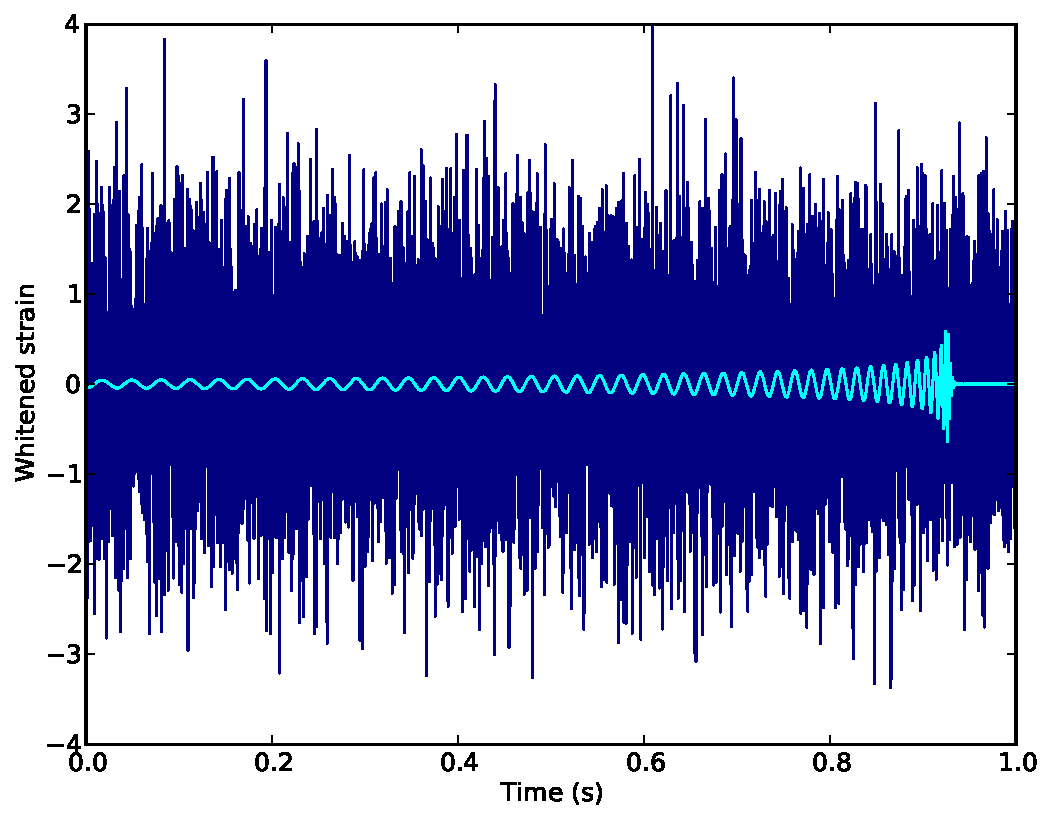
\includegraphics[width=\columnwidth]{figures/waveform.pdf}
\caption[Whitened noise-free timeseries of a \ac{BBH} signal]{A whitened noise-free timeseries of a \ac{BBH} signal sampled at $8192$~Hz with component masses $m_{1}=41.86\mathrm{M}_{\odot}$ and $m_{2}=6.65\mathrm{M}_{\odot}$ with optimal \ac{SNR} $\optsnr=8$ (cyan). The dark blue timeseries shows the same gravitational-wave signal with additive whitened Gaussian noise of unit variance. This latter timeseries is representative of the datasets used to train, validate, and test the deep neural network.\label{fig:waveform}}
\end{figure}

%
% define the CNN structure 
% 
\section{The Deep Network Approach}
%
% introduce convolutional neural networks
%
In our model, we use a variant of a deep learning algorithm called a 
\ac{CNN}~\cite{726791} composed of multiple layers (See Ch.~\ref{ch:chap_2}). 
The input layer holds the raw pixel values of the sample image which, in our 
case, is a 1-dimensional timeseries vector. The weight and bias 
parameters of the network are also in 1-dimensional vector 
form. This is opposed to the traditional 2-dimensional vector form more 
commonly used by \ac{ML} practitioners when applying \ac{CNN}s towards 
2-dimensional image analysis. We do not use a 2-dimensional 
vector form because our inputs are 1-dimensional, thus we would ideally 
like our \ac{CNN} filters to reflect that reality. Each neuron in 
the convolutional layer computes the convolution between the neuron's 
weight vector and the outputs from the layer below it, and then the 
result is summed with the bias vector. Neuron weight vectors are 
updated through an optimisation algorithm 
called back-propogation~\cite{LeCun1998}. Activation 
functions apply an element-wise non-linear operation 
rescaling their inputs onto a specific range and leaving the 
size of the previous layer's output unchanged. Pooling layers 
perform a downsampling operation along the spatial dimensions 
of their input. Finally we have a hidden layer connected to an output layer which
computes the inferred class probabilities. These values are 
input to a loss function, chosen as the 
binary cross-entropy~\cite{tensorflow2015-whitepaper}, defined as
%
% define the loss function
%
\begin{equation} \label{eq:loss} 
f(p,t) =
-\sum_{i\in\text{S}}t_{i}^{\mathrm{S}}\mathrm{log}(p^{\text{S}}_{i})-\sum_{i\in\text{N}}t_{i}^{\mathrm{N}}\mathrm{log}(p^{\text{N}}_{i}), 
\end{equation}
%
where $p^{\text{S/N}}_{i}$ is the predicted probability of the class signal+noise (S) or noise-only (N) and $t^{\text{S/N}}_{i}$ is the true value 
for the $i$'th training sample. The loss function is minimised when input data samples are assigned the correct class with the highest confidence. 

%
% describe the network choices that we have
%
In order to optimise a network, multiple hyper-parameters must be tuned. 
We define hyper-parameters as parameters that we are free to 
choose. Such parameters include the number and type of network layers, 
the number of neurons within each layer, the size of the neuron 
weight vectors, the max-pooling parameters, the type of activation 
functions, the preprocessing of input data, the learning rate, and the 
application (or otherwise) of specific deep learning techniques. We 
begin the process with the simplest network that provides a 
discernible level of effective classification. In most 
cases this consists of an input, convolutional, hidden, and 
logistic output layer. The optimal network structure was 
determined through multiple tests and tunings of hyperparameters by 
means of trial and error~\footnote{We have also used multiple other 
hyperparameter optimisation techniques, as introduced in Ch.~\ref{ch:chap_2}, 
in subsequent projects. We tried some of these optimisation schemes 
in Ch.~\ref{ch:chap_4}, but in the end settled on a network design which 
was determined through random trial and error.}.

%
% go into more detail about what we tried in network design
%
Within our optimisation process we experimented with rescaling the input 
data, which we found to have minimal effect on the network performance. The 
reason for this is that our input data is whitened and our 
signals are buried beneath the noise. Therefore our data is effectively 
prescaled on a range $\pm\mathcal{O}(1)$ due to the natural 
variation of Gaussian noise. We also experimented with using 
transfer learning~\cite{5288526} where networks pre-trained on 
high \ac{SNR} datasets are used as starting points for application to 
successively lower \ac{SNR} datasets. We found that there were no 
performance benefits in using this approach compared to training the 
network solely on each \ac{SNR} dataset separately. The network depth was 
adjusted between 2 and 10 convolutional layers. The inclusion of 
dropout (See Sec.~\ref{sec:ml_regularization} of Ch.~\ref{ch:chap_2})
was used within the final 2 hidden layers as a form of 
regularisation to avoid overfitting.

%
% describe how the training itself works to optimise the weights and biases
%
During the training stage an optimisation function (back-propagation) works 
by computing the gradient of the loss function (Eq.~\ref{eq:loss}) with 
respect to the weights of the network for a given training sample, 
then attempting to minimize 
that loss function. The value of the loss is propagated back 
through the network by taking the partial derivative of the loss with respect 
to the weights of the network and applying the chain rule. 
Using the calculated partial 
derivatives, one can then update the weight and bias terms of the network such 
that the loss is minimised.  Back propagation is done over multiple 
iterations where at each iteration the gradients are computed all at once over 
a batch of training samples. We also use Nesterov momentum~\cite{dozat2016incorporating}, which is described by  
%
\begin{equation} \label{eq:nesterov1}
v_{i} = \mu v_{i-1} - \eta \nabla f(\theta_{i-1} + \mu v_{i-1}),
\end{equation}
%
\begin{equation} \label{eq:nesterov2}
\theta_{i} = \theta_{i-1} + v_{i},
\end{equation} \\
%
where $\theta_{i-1}$ are the parameters of the neural network from the 
previous layer, $\theta_{i}$ are the parameters of the current layer 
of the network, $v_{i}$ is the momentum for the current layer, 
$\mu$ is a scalar constant term which determines 
the amount of momentum to apply per gradient update 
(the higher the number, the more momentum), $v_{i-1}$ is the 
momentum term from the previous layer, $\eta$ is the 
learning rate, $\nabla f(\theta_{i-1} + \mu v_{i-1})$ is the 
gradient of the model parameters with respect to the previous 
layer (including the momentum term from the previous layer ($\mu v_{i-1}$)).
There are a variety of 
initialisation schemes for the momentum term in each layer, but prior to 
training, the momentum in each layer is nominally simplified initially 
chosen from a uniform distribution between 0 and 1.
We use a learning rate of $\eta = 0.002$, and the Adam
optimiser~\cite{2014arXiv1412.6980K} 
which is parameterised by a set of user-defined hyperparameters given as: 
$\beta_{1}=0.9$, $\beta_{2}=0.999$, $\epsilon = 10^{-8}$ and a momentum
schedule of $0.004$ (See~\cite{2014arXiv1412.6980K} for 
further details on the function of 
these Adam hyperparameter values). We outline 
the structure of the final neural network architecture 
in Table~\ref{table:network}. We also note that the same 
network structure was used for each \ac{SNR}, but that a separate neural 
network was trained for every \ac{SNR} value.

%
% the CNN ranking statistic
%
The final ranking statistic that we extract from the \ac{CNN} analysis is 
taken from the output layer, composed of 2 neurons, where each neuron 
gives the inferred probability that the input data belongs to the 
noise or signal+noise class respectively. Both neurons
will produce a probability value between 0 and 1 with their sum 
being unity, which is the default behaviour of the 
softmax activation function given by 
%
\begin{equation}
    \mathrm{Softmax(x_i)} = \frac{e^{x_i}}{\sum_j e^{x_j}},
\end{equation}
%
where $e^{x_i}$ is the exponent of the value of one of the 2 output layer 
neurons for class $i$ and 
$\sum_j e^{x_j}$ is a summation over the exponent of both neuron 
output layer values, representing the predictions for all classes. 
The computational time spent on training the network for 
each SNR is $\mathcal{O}(1)$ hour on a single GPU. This one-time 
cost can be compared to the $\mathcal{O}(1 s)$ spent applying the 
trained network to all $25,000$ 1 s test data samples also 
using a single GPU. Therefore at the point of data taking this 
particular analysis can be run at ~$10^{4}$ times faster than real-time.

%
% Reference the loss, dp, lr  figure
%
In Fig.~\ref{fig:loss_curve}, we plot three different quantities 
as a function of training epoch for one of our networks trained 
on \ac{SNR} 8 signals. The top panel shows the loss as a 
function of training epoch, which we see decreases rapidly 
initially and then levels out as training progresses. In the 
middle panel, we show the detection probability (fraction of \ac{GW} 
signals correctly identified by the neural network) as a 
function of training epoch where the training, validation and testing 
detection probability are denoted as the purple, blue and orange curves 
respectively. The goal is to minimize the loss 
function, which will in turn maximise the detection probability of the 
classifier. We see in Fig.~\ref{fig:loss_curve} that as the loss decreases, 
the detection probability increases, indicating the the network is 
performing more accurately as training progresses. We should note here though 
that it does appear that the network is slightly overfitting to the 
training data. This is because the validation/testing detection probability 
curves (blue, orange) are lower than the training probability curve (purple). 
The bottom panel 
shows the learning rate used as a function of training epoch which 
oscillates between $10^{-3}$ and $5 \times 10^{-3}$. 

%
% Small discussion on cyclic learning rate
%
Our learning rate oscilates between a minimum and upper bound because 
we decided to employ a cyclic learning rate
scheduler~\cite{2015arXiv150601186S}. A cyclic learning rate is 
commonly used avoid saddle points, or local minima, in the 
loss function parameter space. Specifically, a learning rate which 
is too low will only apply small updates to the neural network weights and 
thus may get stuck in that saddle point. A cyclic learning rate 
will allow both large and small network weight updates to occur, thus 
increasing the likelihood of breaking out of saddle points. There is 
also the issue of choosing a poor initial learning rate at the beginning 
of training. If our network and/or optimiser is strongly influenced 
by the initial learning rate, we may never see the loss function 
minimised. A cyclic learning rate allows us apply a variety of learning 
rate values over a broad range, thus minimising the chance of choosing 
an inappropriate learning rate.

\begin{figure} 
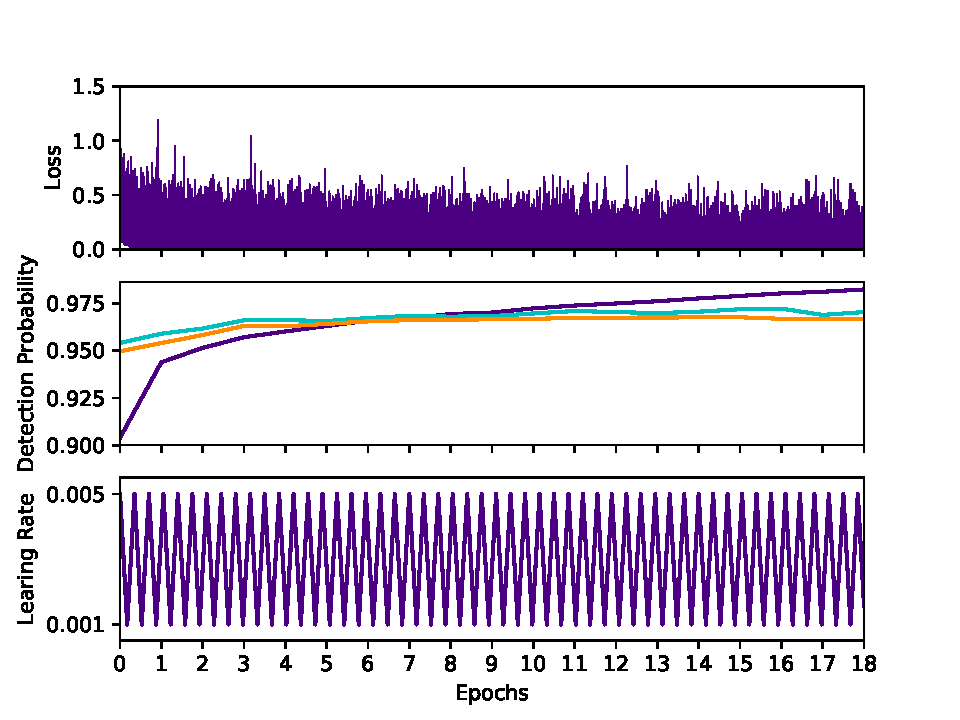
\includegraphics[width=\columnwidth]{figures/matching_matched_filtering_loss.pdf}
\caption[CNN loss, detection probability and learning rate plots illustrate 
how the network's performance is defined as a function of the number of 
training epochs.]{\label{fig:loss_curve} The loss, detection 
probability and learning rate plots (shown above top panel) for 
a network trained on \ac{SNR} 8 signals 
illustrate how the network's performance is defined as a function 
of the number of training epochs. The first initial epochs see an 
exponential decrease in the loss function and then a slowly falling 
values to follow. This indicates that the longer our network is trained, 
a limit with respect to the accuracy is approached. In our case, we 
cyclically adjust the learning rate to oscillate between 
$5 \times 10^{-4}$ and $10^{-3}$ at a constant frequency. The 
detection probability on training samples is represented by 
the purple curve, validation detection probability as the 
blue, and testing detection probability as the orange 
curve.}
\end{figure}

\begin{table}[]
\centering
\begin{tabular}{lccccccccc}
\hline
\hline
Parameter & \multicolumn{9}{c}{Layer}\\
\cline{2-10}
(Option) & 1 & 2 & 3 & 4 & 5 & 6 & 7 & 8 & 9 \\
\hline
Type & C & C & C & C & C & C & H & H & H \\
No. Neurons  & 8  & 8  & 16 & 16 & 32 & 32 & 64  & 64  & 2  \\
Filter Size  & 64 & 32 & 32 & 16 & 16  & 16  & n/a & n/a & n/a  \\
MaxPool Size & n/a & 8 & n/a & 6 & n/a & 4 & n/a & n/a & n/a \\
Drop out  & 0 & 0 & 0 & 0 & 0 & 0 & 0.5 & 0.5 & 0 \\
Act. Func. & Elu & Elu & Elu & Elu & Elu & Elu & Elu & Elu & SMax \\
\hline
\end{tabular}
\caption[CNN optimised network configuration consisting of 6 convolutional layers (C), followed by 3 hidden layers (H).]{The optimised network consisting of 6 convolutional layers (C), followed by 3 hidden layers (H). Max-pooling is performed on the first, fifth, and eighth layer, whereas dropout is only performed on the two hidden layers. Each layer uses an exponential linear unit (Elu) activation function (with range $[-1,\infty]$) while the last layer uses a Softmax (SMax) activation function in order to normalize the output values to be between zero and one so as to give a probability value for each class.\label{table:network}}
\end{table}

%
% define the matched-filter analysis
%
\section{Applying Matched-Filtering}
%
% introduce matched-filtering
%
In order to establish the power of the deep learning approach we must compare 
our results to the standard matched-filtering process used in the 
detection of \ac{CBC} signals~\cite{PhysRevD.85.122006,2013PhRvD..87b4033B}. 
The ranking statistic used in this case is the matched-filter 
\ac{SNR} numerically maximized over arrival time and analytically 
maximised over phase and distance~\cite{Anderson2011}. 
\hunter{Add reference back to chapter 1 if I add in the 
time, phase and amplitude matched filter maximisation derivation.}
By first defining the noise 
weighted inner product as a function of a time shift $\Delta t$ between 
$a$ and $b$ given as,
%
% define the matched-filtering SNR
%
\begin{equation}\label{eq:inner}
(a\mid b)(\Delta t) =
4\int_{f_{\mathrm{min}}}^{\infty}\frac{\tilde{a}(f)\tilde{b}^{*}(f)}{S_{\mathrm{n}}(f)}e^{2\pi i
f\Delta t}\,df,
\end{equation}
%
we can construct the squared matched-filter \ac{SNR} as 
%
\begin{equation}\label{eq:match_filt_snr_squared}
\rho^{2}(\Delta t)=\frac{(s\mid h)^{2}(\Delta t) + 
i(s\mid h)^{2}(\Delta t)}{(h\mid h)}
\end{equation}
%
where $s$ is the data containing noise and a potential signal, and $h$ 
is the noise-free gravitational-wave template and 
$\Delta t = 1/f_{s}$ and $f_s$ is the sampling
frequency~\cite{0264-9381-23-18-002}. 
For a given template this quantity is efficiently computed using the 
\ac{FFT}, where the \ac{FFT} allows the \ac{SNR} to be computed 
for all possible signal arrival times within the observation window with 
cost $N\log{N}$, where $N$ is the number of samples we have~\footnote{
If we didn't use the \ac{FFT}, then the brute force cost would $N^2$ (
correlating the template once costs $N$ operations and then shifting it by one 
bin and doing it again $N$ times.}. The maximum 
\ac{SNR} value from the output \ac{SNR} timeseries, defined by 
Eq.~\ref{eq:match_filt_snr_squared}, is also computed. The subsequent 
step is to further numerically maximize this quantity over a 
collection of component mass combinations. In this analysis a 
comprehensive template bank is generated in the $m_{1},m_{2}$ mass 
space covering our predefined range of masses. We use a 
maximum mismatch of $3\%$ and a lower frequency cutoff of 
$20~\mathrm{Hz}$ using the PyCBC geometric non-spinning template 
bank generation tool~\cite{pycbc-software,0264-9381-33-21-215004}. 
This template bank contained $8056$ individual templates. 

%
% describe the process of what we apply this to
%
When generating an \ac{SNR} timeseries (Eq.~\ref{eq:match_filt_snr_squared}) 
for an input dataset we select $f_{\mathrm{min}}$ according to the 
conservative case in which the signal merger occurs at the 0.95 
fraction of the 1~s timeseries. We therefore select only maximised 
\ac{SNR} timeseries values recovered from within the $[0.75,0.95]$ 
fractional range since this is the parameter space on which the 
\ac{CNN} has been trained. For the practical computation of the 
matched-filtering analysis we take each of the data samples from the 
testing dataset to compute the matched-filter ranking statistic.

%
% Describe the main results of the study
%

%
% a description of the main results
%
\section{Matching Matched Filtering Results}
%
% main introduction to results
%
After tuning the multiple hyper-parameters (Table~\ref{table:network}) 
and training the neural network (Fig.~\ref{fig:loss_curve}), we present 
the results of our \ac{CNN} classifier on a noise versus signal+noise 
sample set. With values of ranking statistics now assigned to each 
test data sample from both the \ac{CNN} and matched-filtering 
approaches, and having knowledge of the true class associated with 
each sample, we may now construct \ac{ROC} curves to compare performance. 

%
% introduce the confusion matrix results
%
A standard method for displaying the accuracy of a classifier is 
through a confusion matrix in which the number of samples of each 
true class identified as every possible class are listed in a 
square matrix. A fully diagonal matrix would imply no incorrectly 
classified samples and a uniform matrix would 
imply no classification power (with the 
stipulation that there are equal numbers of testing samples 
in each class). Classification, within the context of a confusion 
matrix, is defined as when the neural network predicts a value 
of greater than $p=0.5$ for a single class. We also highlight that this 
can't be done with the matched filtering approach and thus only 
show results from the \ac{CNN} in the confusion matrix. In
Fig.~\ref{fig:confusion} we show results for the \ac{CNN} approach 
from which we highlight the overall accuracy 
(the ratio of incorrectly identified samples to the total number of 
samples) is $[51.88\%,65.51\%,85.63\%,96.66\%,99.41\%,99.99\%]$ 
at $\rho_{\mathrm{opt}}=[2,4,6,8,10,12]$, for a fixed detection 
threshold of $p=0.5$. 
We highlight that the measure of \ac{CNN} accuracy 
illustrated by Fig.~\ref{fig:confusion} is 
interesting in general, but not useful for 
us in practice since we want to maximise the true alarm at a fixed 
false alarm value.

%
% confusion matrix plot
%
\begin{figure}[]
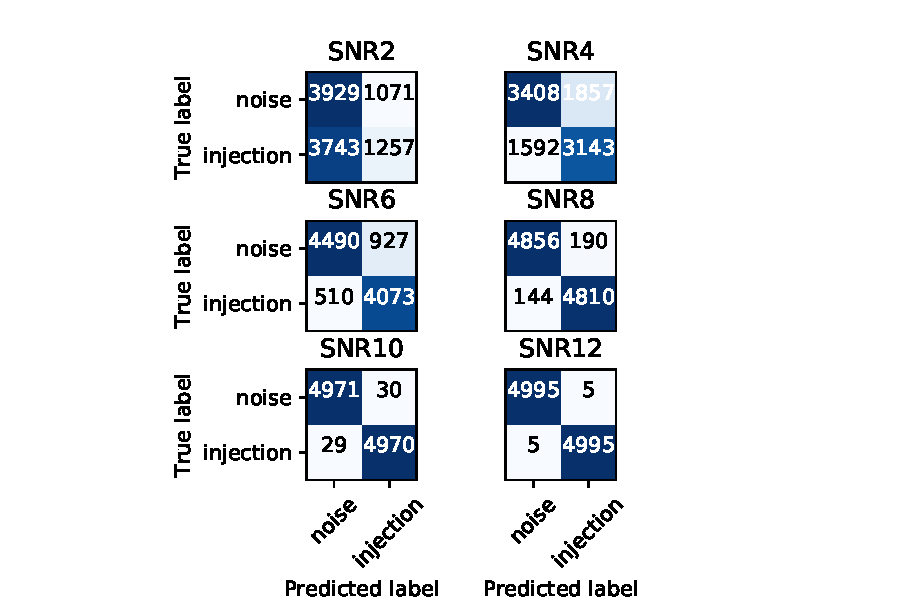
\includegraphics[width=\columnwidth] {figures/confusion_matrix.pdf}
\caption[Confusion matrices for testing datasets containing signals with 
optimal SNR $\rho_{\mathrm{opt}}=2,4,6,8,10,12$]{Confusion matrices for 
testing datasets containing signals with optimal \ac{SNR}
(Given in Eq.~\ref{eq:snr}) $\rho_{\mathrm{opt}}=2,4,6,8,10,12$. 
Numerical values superimposed within matrix elements represent the number of 
samples that were of true class indicated by the $y$-axis label but 
identified as the corresponding $x$-axis label. For our 2 class 
system these are equivalent to the numbers of true alarm, true dismissal, 
false dismissal, or false alarm, for a fixed detection threshold 
of $p=0.5$. The accuracy
percentages for all injection SNR values are listed as follows: $51.86\%$ at
$\rho_{\mathrm{opt}}=2$, $65.51\%$ at $\rho_{\mathrm{opt}}=4$, 
$85.63\%$ at $\rho_{\mathrm{opt}}=6$, $96.66\%$ at
$\rho_{\mathrm{opt}}=8$, $99.41\%$ at $\rho_{\mathrm{opt}}=10$ and $99.99\%$ at
$\rho_{\mathrm{opt}}=12$.\label{fig:confusion}}
\end{figure}

%
% describe ROC curves
%
In Fig.~\ref{fig:ROC_curves} we compare our \ac{CNN} results to that 
of matched-filtering. Given the ranking statistic from a particular 
analysis and defining a parametric threshold value on that statistic 
we are able to plot the fraction of noise samples incorrectly 
identified as signals (\ac{FAP}) versus the fraction of signal 
samples correctly identified (\ac{TAP}). These curves are defined 
as \ac{ROC} curves and a ranking statistic is deemed superior to 
another if at a given \ac{FAP} it achieves a higher detection 
probability. Our results show that the \ac{CNN} approach closely 
matches the sensitivity of matched-filtering for all test 
datasets across the range of \ac{FAP}s explored in this 
analysis\footnote{We are limited to a minimal \ac{FAP} of 
$\sim 10^{-4}$ due to the limited number of 
testing samples used.}. 
%It is not surprising to see that the 
%matched-filtering method using the optimal template consistently 
%performs better than both the nominal match-filtering method and 
%our deep learning classifier~\chris{NO. we don't show the optimal template result anywhere. Maybe we did at one point in the past. Either add those results to the figures or remove this reference.}. However, what is considerable is the comparison between the nominal~\chris{drop this "nominal" business if you are also going to drop the "optinal" template analysis.} matched-filtering and the deep learning classifier detection probability curves. 
It can clearly be seen that our classifier also exceeds the 
performance of the matched-filtering method at optimal 
\ac{SNR} $\rho_{\mathrm{opt}}=2,4,6$. This is an interesting result 
and is not entirely unexpected given that matched-filtering is not 
expected to be completely
optimal~\cite{2008arXiv0804.1161S,2021arXiv210403961Y}.

%
% show ROC curves
%
\begin{figure}[]
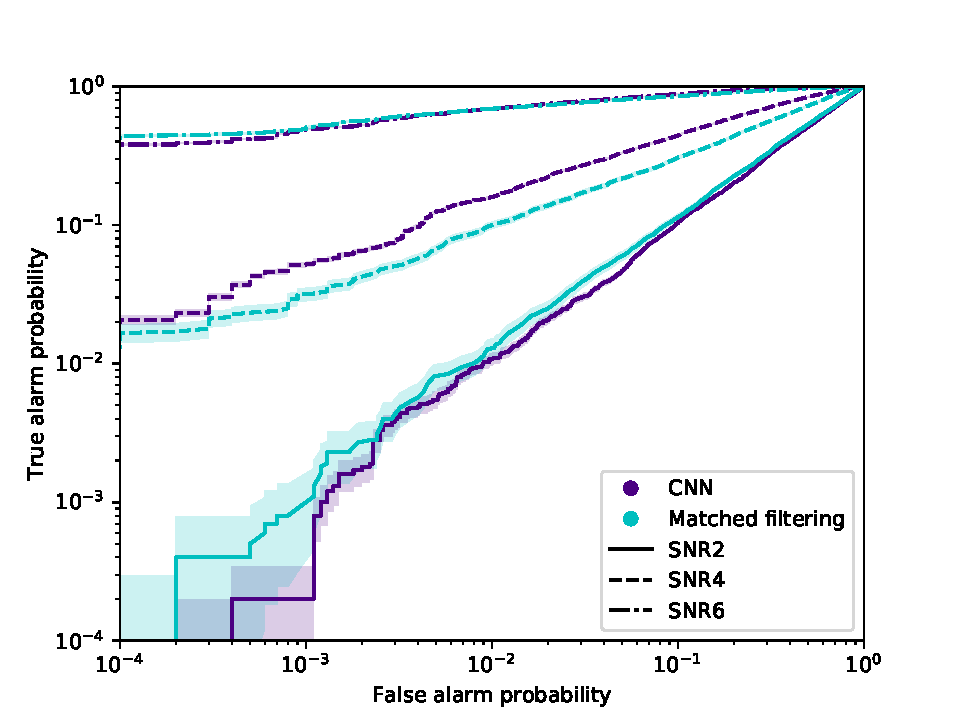
\includegraphics[width=\columnwidth] {figures/ROC_curves.pdf}
\caption[Receiver operating characteristic curves for test datasets containing signals with optimal signal to noise ratio, $\rho_{\mathrm{opt}}=2,4,6$]{The \ac{ROC} curves for test datasets containing signals with optimal \ac{SNR}, $\rho_{\mathrm{opt}}=2,4,6$. We plot the true alarm probability versus the false alarm probability estimated from the output of the \ac{CNN} (purple) and matched-filtering (cyan) approaches. Uncertainties in the true alarm probability correspond to 1-$\sigma$ bounds assuming a binomial distribution.} \label{fig:ROC_curves} 
\end{figure}

%
% finally discuss the efficiency plot
%
We can make an additional direct comparison between approaches by fixing a 
\ac{FAP} and plotting the corresponding \ac{TAP} versus the optimal 
\ac{SNR} of the signals in each test dataset. We show these efficiency 
curves in Fig.~\ref{fig:efficiency_curve} at \ac{FAP}s 
$10^{-1},10^{-2},10^{-3}$ for both the \ac{CNN} and matched-filtering 
approaches. We again see very good agreement between the approaches at all 
\ac{FAP}s with the \ac{CNN} sensitivity exceeding that of the 
matched-filter approach at low \ac{SNR} and high \ac{FAP}. 
Conversely we see the matched-filter sensitivity marginally exceeds 
the \ac{CNN} at high \ac{SNR} and low false alarm probability. 
This latter discrepancy could be mitigated by increasing the number 
of training samples in the CNN approach.

%
% show efficiency curve
%
\begin{figure}[]
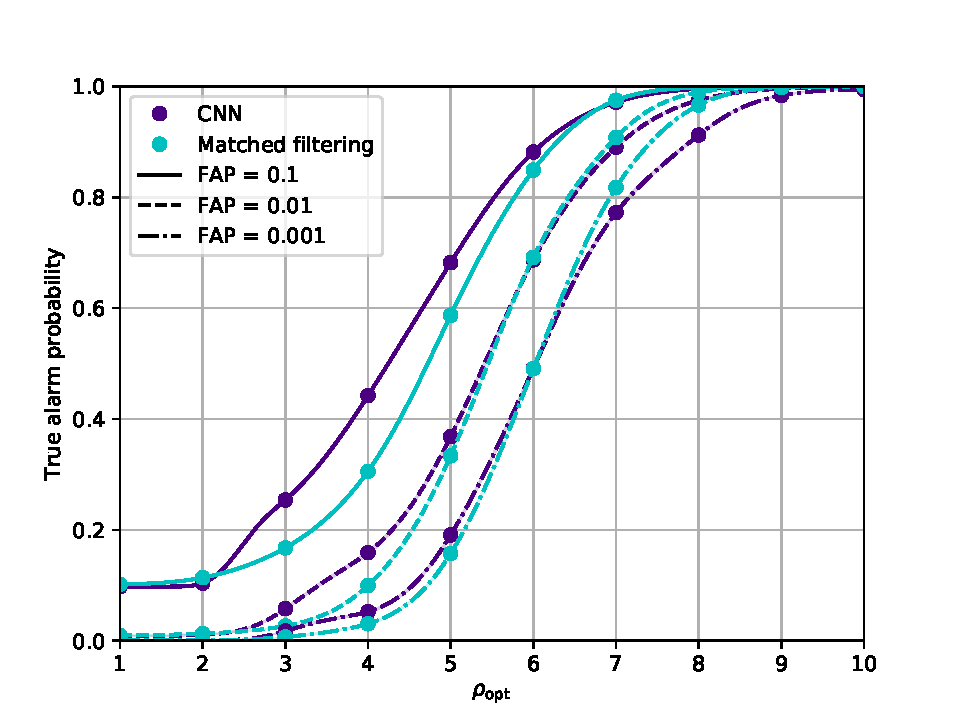
\includegraphics[width=\columnwidth] {figures/efficiency.pdf}
\caption[Efficiency curves comparing the performance of the CNNs~\chris{use acronym package - or maybe it doesn't work with short figure titles, BTW this short figure title isn't very short} and matched-filtering approaches for false alarm probabilities $10^{-1}$ (solid), $10^{-2}$ (dashed), $10^{-3}$ (dot-dashed).]{Efficiency curves comparing the performance of the \ac{CNN} and matched-filtering approaches for false alarm probabilities $10^{-1}$ (solid), $10^{-2}$ (dashed), and $10^{-3}$ (dot-dashed). The true alarm probability is plotted as a function of the optimal \ac{SNR} for the \ac{CNN} (purple) and the
matched-filtering (cyan) analyses. Solid dots indicate at which \ac{SNR} values analyses were performed and light shaded areas are representative of 
the statistical uncertainties in the curves (which are all smaller than the 
line thicknesses).\label{fig:efficiency_curve}} 
\end{figure}

%
% Summarise what you did, note key equations and specific results. If there is
% a main numerical result, quote it here. Then go back and make sure the
% abstract contains the most important results. Say what’s next
%
\section{Matching Matched Filtering Conclusions}\label{sec:mmf_conclusions} 
%
% summary of what we did
%
We have demonstrated that deep learning, when applied to \ac{GW}
timeseries data, is able to closely reproduce the results of a 
matched-filtering analysis in Gaussian noise. We employ a 
deep convolutional neural network with rigorously tuned 
hyperparameters and produce an output that returns a ranking 
statistic interpreted as the inferred probability that data contains a 
signal. Matched-filtering analyses are often described as 
the optimal approach for signal detection in Gaussian 
noise, but in reality are only close to
optimal~\cite{2008arXiv0804.1161S,2021arXiv210403961Y}. By building a 
neural network that is capable of matching the efficiency of matched 
filtering we answer a fundamental question regarding the applicability 
of neural networks for \ac{GW} data analysis. 

%
% Non Gaussian noise
%
In practice, searches for transient signals in \ac{GW} data are strongly 
affected by non-Gaussian noise artefacts. To account for this, 
standard matched-filtering approaches are modified to include 
carefully chosen changes to the ranking
statistic~\cite{PhysRevD.71.062001,0004-637X-849-2-118} together with 
the excision of poor quality data~\cite{1710.02185, 0264-9381-33-13-134001}. 
Our analysis represents a starting point from which a deep network 
can be trained on realistic non-Gaussian data. Since the 
claim of matched-filtering near optimality is applicable only in the 
Gaussian noise case, there exists the potential for deep networks 
to exceed the sensitivity of existing matched-filtering 
approaches in real data.

%
% On the use of multiple networks
%
We should also note that one of the downsides of our 
approach has been the use of separate 
neural networks for each \ac{SNR} value. This could easily 
be overcome by simply training a single \ac{CNN} model using a training set 
which contains \ac{GW} waveforms with multiple \ac{SNR} values. In fact, 
it was shown in~\cite{PhysRevD.100.044009} that single networks can generalise 
well to different \ac{SNR} values. 

%
% Other sources and final statement
%
In this work we have presented results for \ac{BBH} mergers, however, 
this method could be applied to other merger types, such as 
\ac{BNS} (as was shown in~\cite{PhysRevD.102.063015,KRASTEV2020135330}) 
and \ac{NSBH} signals. 
This supervised learning approach can 
also be extended to other well modelled \ac{GW} targets such as the 
continuous emission from rapidly rotating non-axisymmetric \ac{NS}s (as 
was done by~\cite{PhysRevD.100.044009}). Moreover, unsupervised 
approaches have the potential to be powerful detection tools in 
searches for unmodelled burst-like \ac{GW} signals, where it was 
shown in~\cite{2021CQGra..38o5005M} that \acp{GAN} could be 
used for such a task. Finally we 
mention the possibilities for parameter estimation~\cite{GEORGE201864}
~\hunter{More point estimate citations} where 
in the simplest cases an output regression layer can return 
point estimates of parameter values. As was exemplified in the 
case of GW170817~\cite{PhysRevLett.119.161101}, rapid detection confidence 
coupled with robust and equally rapid parameter estimates is 
critical for \ac{GW} multi-messenger astronomy. 

%
% Concluding remarks and transition
%
Since the publication of this paper, a lot has changed in the field of 
\ac{ML} for \ac{GW} astronomy. Many of the outstanding problems we outlined 
here in the conclusions have now been largely solved, such as applying 
deep learning towards other signal types~\cite{KRASTEV2020135330,PhysRevD.102.063015,2021CQGra..38o5005M,2021arXiv210513664B,Cuoco_2020}.\hunter{Need to finish this paragraph.}
In the following chapter 
(Ch.~\ref{ch:chap_5}) we will show how we have used \acp{CVAE} for the purpose 
of generating rapid Bayesian posterior parameter estimates which is 
consistent with other traditional sampling techniques. 

\chris{OK, obviously a very nice chapter. The things to be careful about in addition to my specific comments are the elements in the introduction and conclusion of this chapter that are now out of date. You *could* simply keep them as they are as a historical record of the time. However, that might not fly with your examiners. I would recommend updating these sections to just make sure that you aren't saying completely incorrect things or if you are referring to things that could be dne in the future when they have now actually been done, e.g., the CW stuff you talk about at the very end.}

\chris{Regarding showing any other results. ONLY if you could do things easily, I would be interested in the interpretibility aspects of this chapter. Could you make plots of filters and or layer outputs? It might prove insightful?}

\chris{Additionally, the stand out aspect of this work is how far we've advanced since we wrote it. You make the statement (and a referee might pick up on this) that there is lots of work still to be done on this topic. It begs the question "why didn't we do it?". Rather than actually doing more analysis for this chapter I think that you should add something in the conclusions (a paragraph or 2) about what has happened since this paper was published with regards to CBC detection using ML. You also want to use the final paragraph to segway into the topic of the next chapter on the more challenging topic of PE.}
